\documentclass[11pt,a4paper]{article}
\usepackage[utf8]{inputenc}
\usepackage[T1]{fontenc}
\usepackage{graphicx,booktabs,amsmath}
\usepackage[margin=2.5cm]{geometry}
\usepackage[hidelinks]{hyperref}
\usepackage[font=small,labelfont=bf]{caption}
\setlength{\emergencystretch}{2em}
\graphicspath{{../../figures/pa1/}}
\title{Employee Attrition Prediction Using Non-Probabilistic Classification and Feature Selection}
\author{Adolfo Borrego Gonz\'alez}
\date{Practical Application 1 --- Machine Learning}
\begin{document}
\maketitle
\begin{abstract}
Employee attrition is studied as a binary supervised classification problem using 1,470 observations from the IBM HR Analytics Employee Attrition \& Performance dataset. K-NN, Decision Tree, Support Vector Machine and Neural Network classifiers are compared using all valid predictors, a univariate filter, an mRMR-inspired multivariate filter and a forward-selection wrapper. Predictive performance is estimated through stratified 10-fold cross-validation, with preprocessing and selection fitted within each outer training fold; the wrapper uses internal five-fold selection. The complete representation with the Neural Network obtains the highest mean F1-score (0.4738) and balanced accuracy (0.6765). Reducing 51 transformed features to 15 benefits some classifiers, particularly K-NN under univariate and wrapper selection, but does not improve the strongest full-feature configuration. Repeated selection of original variables supports contextual interpretation of the reduced representations.
\end{abstract}
\section{Introduction}
Employee attrition describes employees leaving an organisation. In this application, recorded employee characteristics are used to distinguish employees who leave from those who remain, giving a supervised binary classification task. The analysis concerns associations in the available data rather than explanations of individual decisions to leave.

Feature selection can reduce dimensionality, remove irrelevant or redundant information and make the retained employee characteristics easier to interpret. These potential benefits need to be assessed against predictive performance: a smaller representation need not preserve all useful information.

The objective of Practical Application 1 is to compare non-probabilistic classification models under four representations: all valid predictors, univariate filter selection, multivariate filter selection and wrapper selection. The research question is: \emph{Which employee characteristics are most relevant for predicting employee attrition, and how does feature selection affect the performance of non-probabilistic classification models?}

\section{Problem Description}
The IBM HR Analytics Employee Attrition \& Performance dataset contains 1,470 employee observations and 35 original columns, including the binary target \texttt{Attrition}. Its distribution is summarised in Table~\ref{tab:dataset}. The dataset is distributed through Kaggle~\cite{ibmhr}. Predictors cover demographics (age and marital status), professional attributes (department and job role), compensation (monthly income and stock options), satisfaction and involvement, experience (working years and company tenure), and working conditions (overtime and business travel).

\begin{table}[htbp]
\centering
\caption{Dataset characteristics and target distribution.}
\label{tab:dataset}
\begin{tabular}{lr}
\toprule
Characteristic & Value \\
\midrule
Observations & 1,470 \\
Original columns, including target & 35 \\
Valid original predictors after removal & 30 \\
Numerical / categorical predictors & 23 / 7 \\
Missing values & 0 \\
\texttt{No}: employee remains & 1,233 (83.88\%) \\
\texttt{Yes}: employee leaves & 237 (16.12\%) \\
\bottomrule
\end{tabular}
\end{table}

The minority class is \texttt{Yes}, so accuracy alone does not adequately describe attrition detection. The identifier \texttt{EmployeeNumber} and the constant columns \texttt{EmployeeCount}, \texttt{Over18} and \texttt{StandardHours} are removed during preprocessing. With 30 valid predictors and 1,470 observations, the dataset exceeds the assignment's minimum of 15 variables and 100 observations.

\section{Methodology}
\subsection{PA1: Non-Probabilistic Classification}
\subsubsection{Data Preprocessing}
The four non-predictive columns identified above are removed, leaving 30 original predictors. No imputation is needed because there are no missing values. The target is encoded as \texttt{No}=0 and \texttt{Yes}=1. The 23 numerical predictors are standardised using \texttt{StandardScaler}; the seven categorical predictors are encoded using \texttt{OneHotEncoder} with \texttt{handle\_unknown="ignore"}. Integer variables representing ordinal levels retain their ordered numerical representation. The complete encoded representation contains 51 transformed features.

A scikit-learn \texttt{Pipeline}~\cite{sklearn} combines preprocessing, optional selection and classification. Fitted preprocessing from structural inspection is not reused for evaluation. Transformations and selectors are fitted on each outer training fold, and then applied to its held-out fold.

\subsubsection{Classification Algorithms}
Four classifiers are used: K-NN classifies from neighbouring observations; Decision Tree uses successive feature splits; SVM constructs a separating decision boundary; and the Neural Network learns a multilayer representation for classification. The implementations are \texttt{KNeighborsClassifier()}, \texttt{DecisionTreeClassifier} (random seed 42), \texttt{SVC()} and \texttt{MLPClassifier} (random seed 42; maximum 2,000 iterations). Other parameters remain at their defaults. The tree is scikit-learn's implementation, not an exact implementation of ID3 or C4.5. These default or minimal configurations are kept consistent across representations to isolate the effect of selection. Hyperparameters are not tuned, and no resampling or class weighting is applied.

\subsection{Shared Evaluation Protocol and Metrics}
\label{sec:evaluation}
Every configuration is evaluated using \texttt{StratifiedKFold} with ten shuffled folds and random seed 42. Stratification approximately preserves class proportions. Each outer held-out fold is excluded from fitting preprocessing, selecting features and training the classifier, providing an honest estimate for each fixed configuration. Reported scores are arithmetic means of the ten held-out-fold scores.

Accuracy measures the proportion of correct predictions. Precision (positive predictive value) measures the proportion of predicted attrition cases that are positive; recall (sensitivity) measures the proportion of actual attrition cases detected. Specificity measures the proportion of negative cases correctly identified. F1-measure is the harmonic mean of precision and recall. Positive-class metrics refer to \texttt{Attrition=Yes}. PA1 records accuracy, precision, recall, F1 and balanced accuracy; the latter averages sensitivity and specificity and is retained as a supplementary PA1 measure.

PA2 reports accuracy, precision, recall, specificity, F1, area under the ROC curve (AUC), and Brier score. AUC evaluates discrimination across decision thresholds. Brier evaluates squared error in the complete predicted class-probability vector:
\[
 B=\frac{1}{n}\sum_{i=1}^{n}\sum_{c\in\{0,1\}}
 \left(p_{ic}-\mathbf{1}\{y_i=c\}\right)^2.
\]
Lower values indicate better probability predictions. This implementation is twice the binary Brier score computed from the positive-class probability alone. Brier reflects both calibration and discrimination, rather than calibration alone. Balanced accuracy is not a primary PA2 metric. Predictions use the implemented classifiers' default decision rules; thresholds are not optimised for recall.

\subsection{PA1: Feature Selection Strategies}
\paragraph{All Features.} The baseline pipeline applies preprocessing directly followed by the classifier, retaining all valid original predictors and their 51 transformed features.

\paragraph{Univariate Filter.} After preprocessing, \texttt{SelectKBest} with \texttt{f\_classif} and $k=15$ retains the 15 transformed features with the highest individual ANOVA F-scores. It assesses association with the target separately for each feature~\cite{selectiondocs}.

\paragraph{Multivariate Filter.} The existing custom greedy selector retains 15 transformed features. It first selects the feature with the greatest estimated mutual information with the target. Subsequently it maximises target mutual information minus the mean absolute Pearson correlation with already selected features. Mutual information is computed using \texttt{mutual\_info\_classif} with random seed 42. This is an mRMR-inspired relevance--redundancy implementation~\cite{mrmr}, rather than a canonical library implementation of mRMR: redundancy is measured by correlation rather than mutual information.

\paragraph{Wrapper.} \texttt{SequentialFeatureSelector} performs forward selection of 15 transformed features using a \texttt{DecisionTreeClassifier} with random seed 42, F1 scoring and internal five-fold CV~\cite{selectiondocs}. The same tree-based selection procedure precedes each of the four final classifiers. Selection is nested within the outer ten-fold evaluation: inner CV chooses the subset, while outer held-out folds estimate predictive performance. In the existing implementation, preprocessing is fitted on the outer training fold before the selector's inner CV; it is not refitted within each inner split. The outer test fold remains excluded throughout.

For interpretation only, separate selector pipelines are fitted to the full dataset to export selected-feature lists. These fits do not generate the reported predictive scores. Their overlap describes agreement across the three strategies in these descriptive fits, rather than selection frequency across CV folds. One-hot categories are mapped back to their original variables.

\subsection{PA2: Probabilistic Classification}
\subsubsection{Model-Specific Representations}
PA2 retains the same 30 valid original predictors and target. One representative implementation is used per family. Mixed Naive Bayes estimates Gaussian class-conditional distributions for continuous predictors and discrete class-conditional probabilities with Laplace smoothing ($\alpha=1$) for ordinal and nominal predictors. It combines these contributions under conditional independence given the class.

Logistic Regression models the log-odds of attrition as an additive function of its transformed predictors. Its pipeline applies \texttt{StandardScaler} to continuous and ordinal variables and \texttt{OneHotEncoder} with one reference category to nominal variables. \texttt{LogisticRegression} uses a maximum of 2,000 iterations and random seed 42, with remaining parameters at defaults.

LDA and QDA model class-conditional distributions with shared and class-specific covariance matrices, respectively. Their pipelines standardise numerical/ordinal predictors and retain one numerically encoded column per nominal predictor, avoiding the rank deficiency introduced by expanded dummy variables. These nominal codes do not imply a meaningful order; their numerical use is a representation limitation. The implementations are \texttt{LinearDiscriminantAnalysis()} and \texttt{QuadraticDiscriminantAnalysis()}. Thus, the families do not receive an identical transformed matrix. Every representation is fitted using training data only.

\subsubsection{Feature Selection on Original Predictors}
\paragraph{All Features.} All 30 valid original predictors are retained before model-specific preprocessing.

\paragraph{Univariate Filter.} A type-aware selector evaluates continuous predictors with ANOVA F-statistics and ordinal/nominal predictors with mutual information. Scores are standardised separately within these two families because their scales differ. The 15 highest-ranked original predictors are retained inside each training fold, before model-specific transformation.

\paragraph{Multivariate Filter.} Correlation-based Feature Selection (CFS) evaluates subset relevance to the target and redundancy between predictors using Symmetrical Uncertainty. Continuous variables are discretised into up to five quantile bins using training data only for this criterion; selected predictors retain their original values for classification. For a subset of size $k$, the merit is
\[
 M=\frac{k\overline{SU}_{Xy}}
 {\sqrt{k+k(k-1)\overline{SU}_{XX}}},
\]
where the averages describe predictor--target association and pairwise predictor redundancy. Greedy forward search considers up to 15 original predictors and retains the subset with the highest merit found. This CFS procedure differs from PA1's mRMR-inspired selector.

\paragraph{Wrapper.} Classifier-specific sequential forward selection searches up to 15 original predictors and retains the subset with the highest internal mean F1. Each classifier conducts its own search in each outer training fold. Internal stratified five-fold CV evaluates candidate model pipelines, refitting preprocessing within each inner training split. The selected pipeline is then fitted on the outer training data and evaluated on its held-out fold using the shared ten-fold protocol. Feature search and final performance estimation are therefore separated; PA1's common tree-based wrapper is not reused.

Separate full-data PA2 filter fits are descriptive only. Fold-level selections are also recorded to assess recurrence under the evaluation protocol, providing information distinct from PA1's descriptive agreement counts.

\subsubsection{Metaclassifiers}
Representative Bagging, AdaBoost and Stacking configurations are evaluated with all valid predictors. Bagging aggregates 100 Decision Trees; AdaBoost combines 100 decision stumps (trees with maximum depth one). Stacking uses Logistic Regression and LDA as base learners and Logistic Regression as the final estimator, trained on internally generated probability predictions with five-fold CV. QDA was excluded from stacking because covariance estimation became numerically unstable in its internal folds.

The ensemble pipelines standardise numerical/ordinal predictors and one-hot encode nominal predictors with a reference category. This shared ensemble representation differs from the standalone LDA/QDA representation. Preprocessing is fitted on each outer training fold before the ensemble's internal operations; it is not independently refitted inside stacking's internal folds. The outer held-out fold remains excluded, so the reported ensemble scores are honest outer-fold estimates, although the internal stacking representation has this limitation. Ensemble variants beyond these representatives are not evaluated.

\section{Results}

\subsection{PA1: Non-Probabilistic Classification}
\subsubsection{Original Feature Set}

With all features, the Neural Network achieves the highest mean F1 (0.4738)
and balanced accuracy (0.6765), with recall 0.4219. SVM obtains the highest
accuracy (0.8653) and precision (0.8363), but recall is 0.2241. Decision Tree
obtains F1 0.3620 and balanced accuracy 0.6206; K-NN obtains F1 0.2115 and
balanced accuracy 0.5577.

\subsubsection{Univariate Filter}

Decision Tree is the highest-F1 classifier under univariate selection, with F1
0.3809 and balanced accuracy 0.6347. Its F1 and balanced accuracy improve
relative to the baseline, as do those of K-NN (F1 0.2968). SVM and Neural
Network obtain lower F1 and balanced accuracy than with all features.

\subsubsection{Multivariate Filter}

The Neural Network has the highest F1 within this strategy, at 0.3902, with
balanced accuracy 0.6341. Decision Tree obtains F1 0.3748. Both K-NN and SVM
score below their baselines; SVM recall falls to 0.0511 and F1 to 0.0910.

\subsubsection{Wrapper}

The Neural Network again has the highest F1 within the strategy (0.3919), with
balanced accuracy 0.6286. K-NN improves from baseline F1 0.2115 to 0.3146 and
from recall 0.1350 to 0.2364. Neither the wrapper Neural Network nor the other
reduced configurations exceed the full-feature Neural Network in F1 or
balanced accuracy.

\subsubsection{Overall Comparison}

Table~\ref{tab:best} lists the highest-F1 configuration within each strategy.
Figure~\ref{fig:f1} shows all 16 F1 comparisons. Among reduced configurations,
Wrapper with Neural Network has the highest F1, whereas Univariate with
Decision Tree has the highest balanced accuracy (0.6347). Every selection
strategy retains 15 of the 51 transformed features, a 70.59\% dimensionality
reduction.

\begin{table}[htbp]
    \centering
    \caption{PA1 highest mean F1 configuration per strategy. BA denotes balanced
    accuracy; all metrics are ten-fold means.}
    \label{tab:best}
    \small
    \setlength{\tabcolsep}{4pt}

    \resizebox{\textwidth}{!}{
        \begin{tabular}{llrrrrr}
\toprule
Strategy & Classifier & Accuracy & Precision & Recall & F1 & BA \\
\midrule
All Features & Neural Network & 0.8490 & 0.5492 & 0.4219 & 0.4738 & 0.6765 \\
Univariate & Decision Tree & 0.7789 & 0.3546 & 0.4219 & 0.3809 & 0.6347 \\
Multivariate & Neural Network & 0.8245 & 0.4501 & 0.3534 & 0.3902 & 0.6341 \\
Wrapper & Neural Network & 0.8401 & 0.5278 & 0.3165 & 0.3919 & 0.6286 \\
\bottomrule
\end{tabular}

    }
\end{table}

\begin{figure}[htbp]
    \centering

    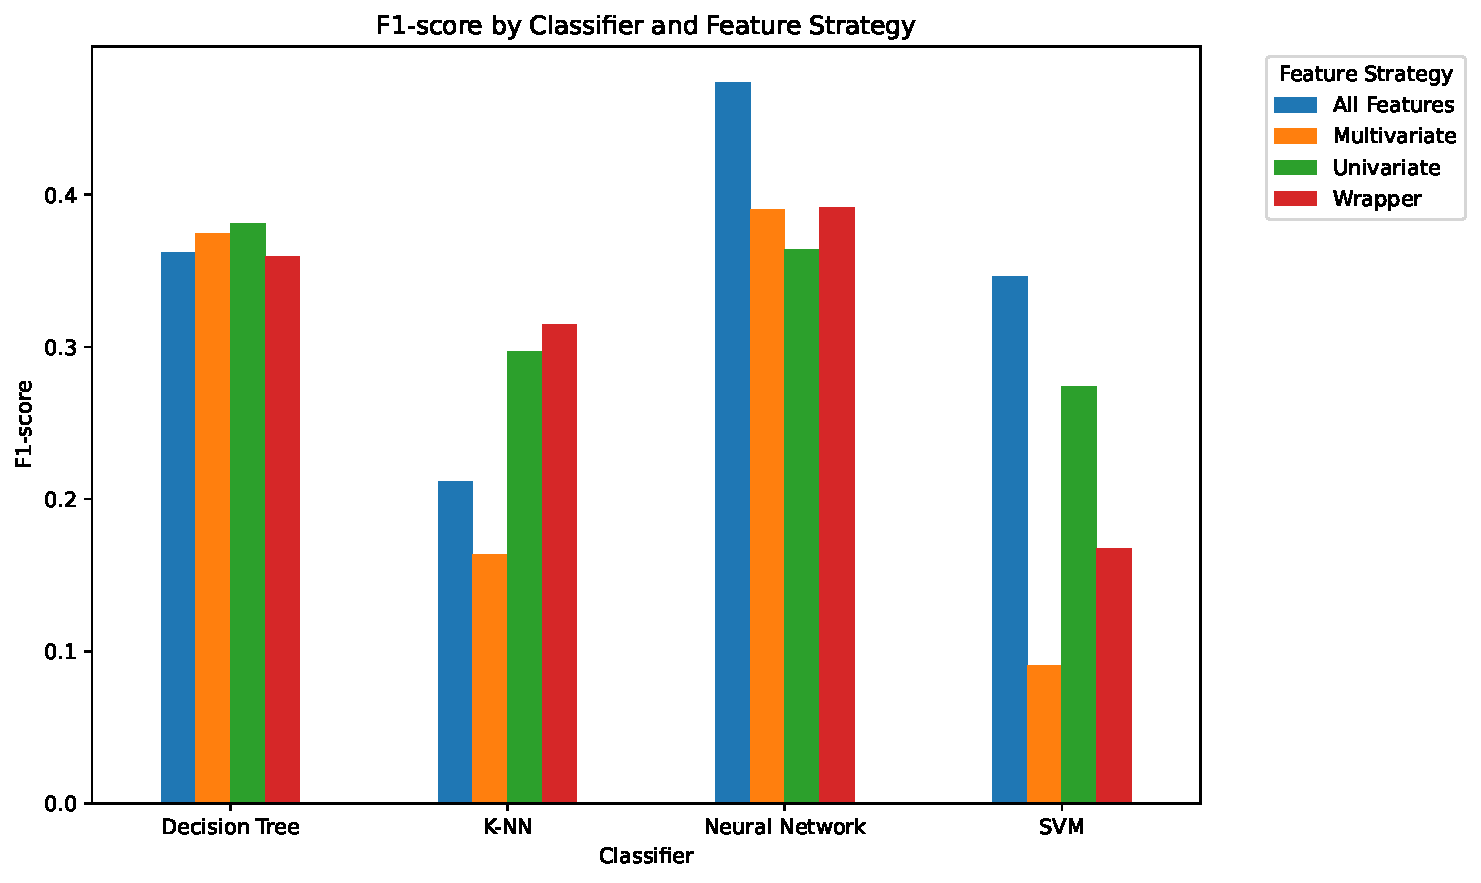
\includegraphics[
        width=0.88\linewidth
    ]{../figures/pa1/f1_comparison.pdf}

    \caption{PA1 mean F1-score by classifier and feature-selection strategy.}
    \label{fig:f1}
\end{figure}

\subsubsection{Selected Variables}

Table~\ref{tab:variables} reports original variables retained by at least two
strategies in the separate full-data interpretation fits. Seven original
variables appear in all three strategies. A categorical variable is counted
as selected when at least one of its dummy features is retained, even when
strategies choose different categories of that variable.

\begin{table}[htbp]
    \centering
    \caption{Agreement between descriptive full-data selections at
    original-variable level. U: univariate; M: multivariate; W: wrapper.}
    \label{tab:variables}
    \small

    \begin{tabular}{lcccc}
\toprule
Original variable & U & M & W & Count \\
\midrule
BusinessTravel & Yes & Yes & Yes & 3 \\
JobInvolvement & Yes & Yes & Yes & 3 \\
JobRole & Yes & Yes & Yes & 3 \\
MaritalStatus & Yes & Yes & Yes & 3 \\
MonthlyIncome & Yes & Yes & Yes & 3 \\
OverTime & Yes & Yes & Yes & 3 \\
StockOptionLevel & Yes & Yes & Yes & 3 \\
Age & Yes & -- & Yes & 2 \\
JobSatisfaction & Yes & Yes & -- & 2 \\
NumCompaniesWorked & -- & Yes & Yes & 2 \\
TotalWorkingYears & Yes & -- & Yes & 2 \\
\bottomrule
\end{tabular}

\end{table}
\subsection{PA2: Probabilistic Classification}
\subsubsection{All Valid Predictors}
Full-feature Logistic Regression obtains the highest F1 among individual probabilistic baselines (0.5373), with accuracy 0.8823, precision 0.7344, recall 0.4259 and specificity 0.9700. It also provides the highest PA2 AUC (0.8375), with Brier 0.1857. Mixed Naive Bayes has the highest recall of all PA2 configurations (0.6453), but lower precision (0.4208), F1 (0.5083), AUC (0.7851) and poorer probability quality (Brier 0.2902). LDA obtains F1 0.4256 and AUC 0.8146; QDA obtains F1 0.3946 and AUC 0.7211.

\subsubsection{Univariate Filter}
Mixed Naive Bayes has the highest F1 within this strategy (0.4600), with recall 0.6033. QDA improves from baseline F1 0.3946 to 0.4240, recall 0.3755 to 0.3924, and AUC 0.7211 to 0.7302, while Brier decreases from 0.2786 to 0.2628. Logistic Regression deteriorates substantially: F1 falls from 0.5373 to 0.3736 and recall from 0.4259 to 0.2708. Thirteen original predictors are retained in all ten folds, including overtime, job level, stock-option level, company tenure, age and monthly income.

\subsubsection{Multivariate Filter}
CFS selects between 3 and 11 original variables per fold (mean 7.8); the separate descriptive full-data fit retains nine. \texttt{JobLevel}, \texttt{OverTime} and \texttt{StockOptionLevel} appear in all ten fold-level subsets, and \texttt{YearsAtCompany} in nine. Mixed Naive Bayes obtains the highest F1 within this strategy (0.3962), with recall 0.3531. The compact subsets therefore lose predictive performance relative to the strongest complete-feature baseline, although its Brier improves from 0.2902 to 0.2386.

\subsubsection{Wrapper}
Logistic Regression obtains the highest F1 among all reduced-feature PA2 configurations (0.4696), with AUC 0.8206 and Brier 0.1976. Mixed Naive Bayes obtains recall 0.4087 and F1 0.4358; QDA obtains F1 0.3848, AUC 0.7165 and Brier 0.2535. Mean selected original-variable counts are 13.1 for Mixed Naive Bayes, 14.6 for Logistic Regression, 13.5 for LDA and 12.9 for QDA. These classifier-specific searches do not outperform the strongest complete-feature baseline.

\subsubsection{Metaclassifiers and Overall Comparison}
Stacking obtains the highest PA2 F1 (0.5394) and lowest Brier (0.1846). Relative to full-feature Logistic Regression, the F1 improvement is marginal, recall is identical (0.4259), and AUC is slightly lower (0.8365 versus 0.8375). AdaBoost obtains F1 0.4676, recall 0.3380 and AUC 0.8314, but its Brier is 0.3773. Bagging obtains F1 0.3407 and recall 0.2362.

Table~\ref{tab:pa2-strategies} summarises the highest-F1 configuration per strategy; Table~\ref{tab:pa2-metrics} identifies the metric-specific leaders. Figure~\ref{fig:pa2-comparison} contrasts F1 with probability-vector error across the evaluated configurations. Rankings use observed cross-validation means and do not establish statistically significant differences.

\begin{table}[htbp]
\centering
\caption{PA2 highest mean F1 configuration per strategy. All scores are ten-fold means; lower Brier is better.}
\label{tab:pa2-strategies}
\small
\setlength{\tabcolsep}{4pt}
\resizebox{\textwidth}{!}{\begin{tabular}{llrrrr}
\toprule
Strategy & Model & Recall & F1 & AUC & Brier \\
\midrule
Metaclassifier & Stacking & 0.425900 & 0.539400 & 0.836500 & 0.184600 \\
All Features & Logistic Regression & 0.425900 & 0.537300 & 0.837500 & 0.185700 \\
Wrapper & Logistic Regression & 0.355100 & 0.469600 & 0.820600 & 0.197600 \\
Univariate & Mixed Naive Bayes & 0.603300 & 0.460000 & 0.763300 & 0.319000 \\
Multivariate & Mixed Naive Bayes & 0.353100 & 0.396200 & 0.761600 & 0.238600 \\
\bottomrule
\end{tabular}
}
\end{table}

\begin{table}[htbp]
\centering
\caption{PA2 leading configurations by objective metric.}
\label{tab:pa2-metrics}
\small
\setlength{\tabcolsep}{4pt}
\begin{tabular}{lllr}
\toprule
Metric & Strategy & Model & Value \\
\midrule
F1 & Metaclassifier & Stacking & 0.539400 \\
Recall & All Features & Mixed Naive Bayes & 0.645300 \\
AUC & All Features & Logistic Regression & 0.837500 \\
Brier & Metaclassifier & Stacking & 0.184600 \\
\bottomrule
\end{tabular}

\end{table}

\begin{figure}[htbp]
\centering
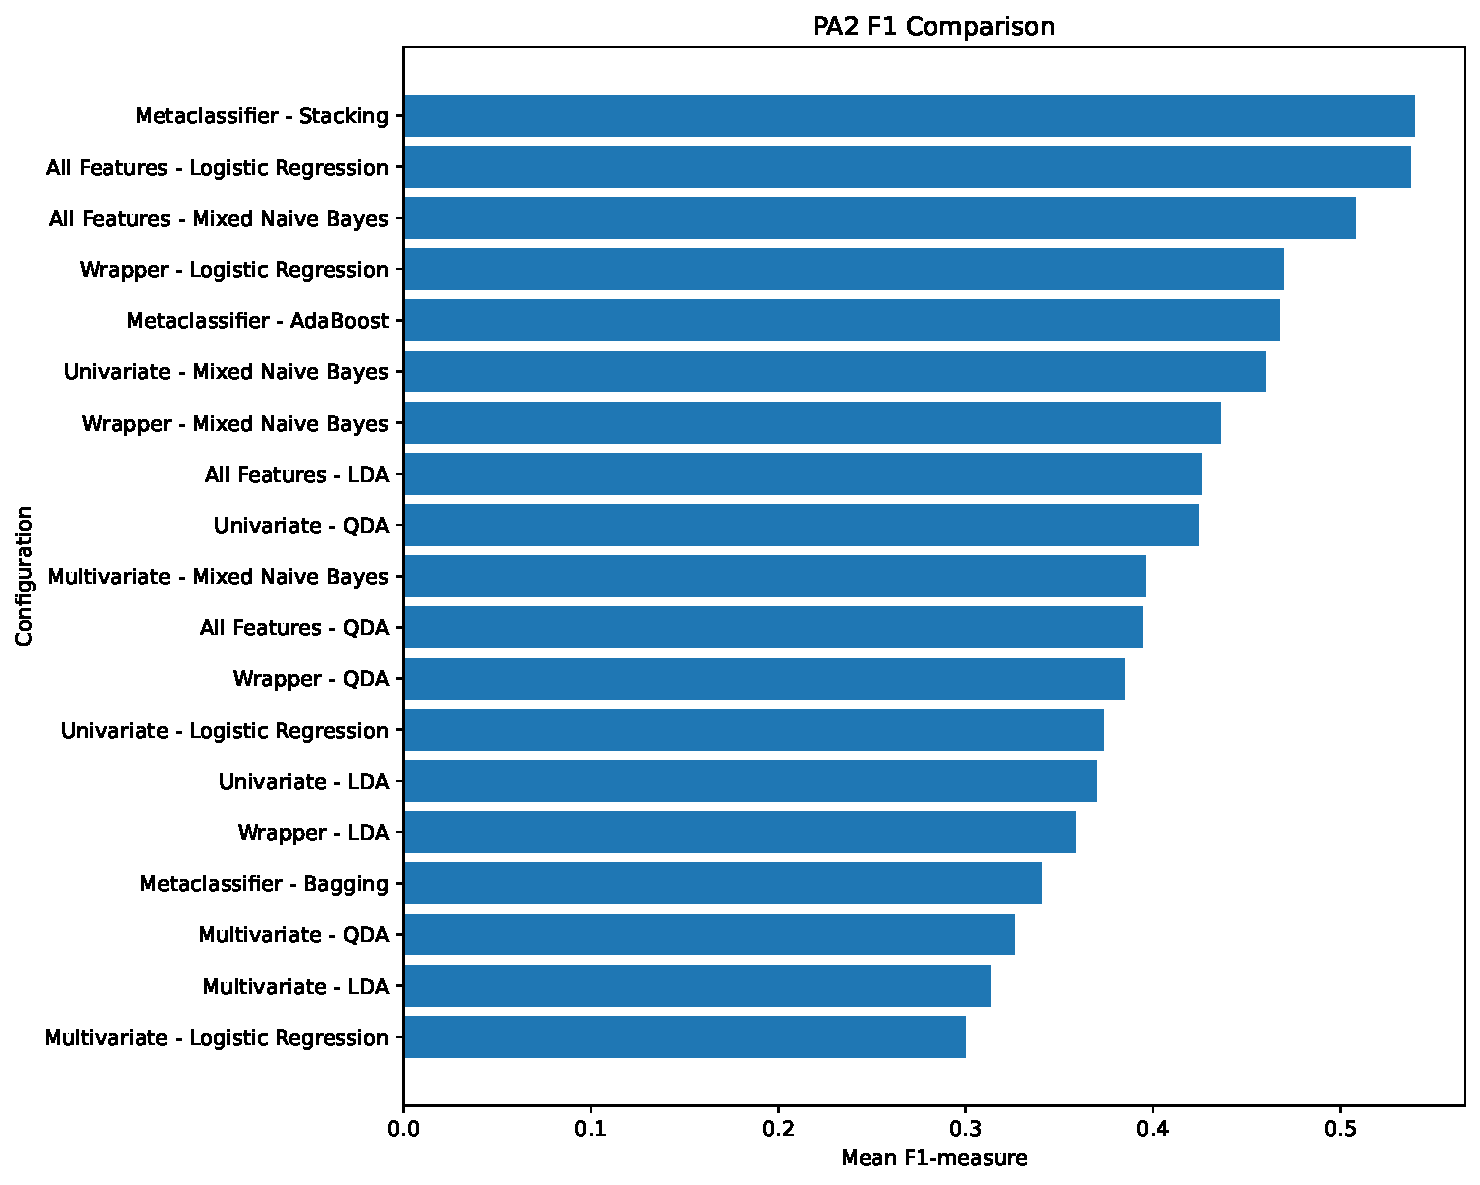
\includegraphics[width=0.76\linewidth]{../figures/pa2/f1_comparison.pdf}
\par\medskip
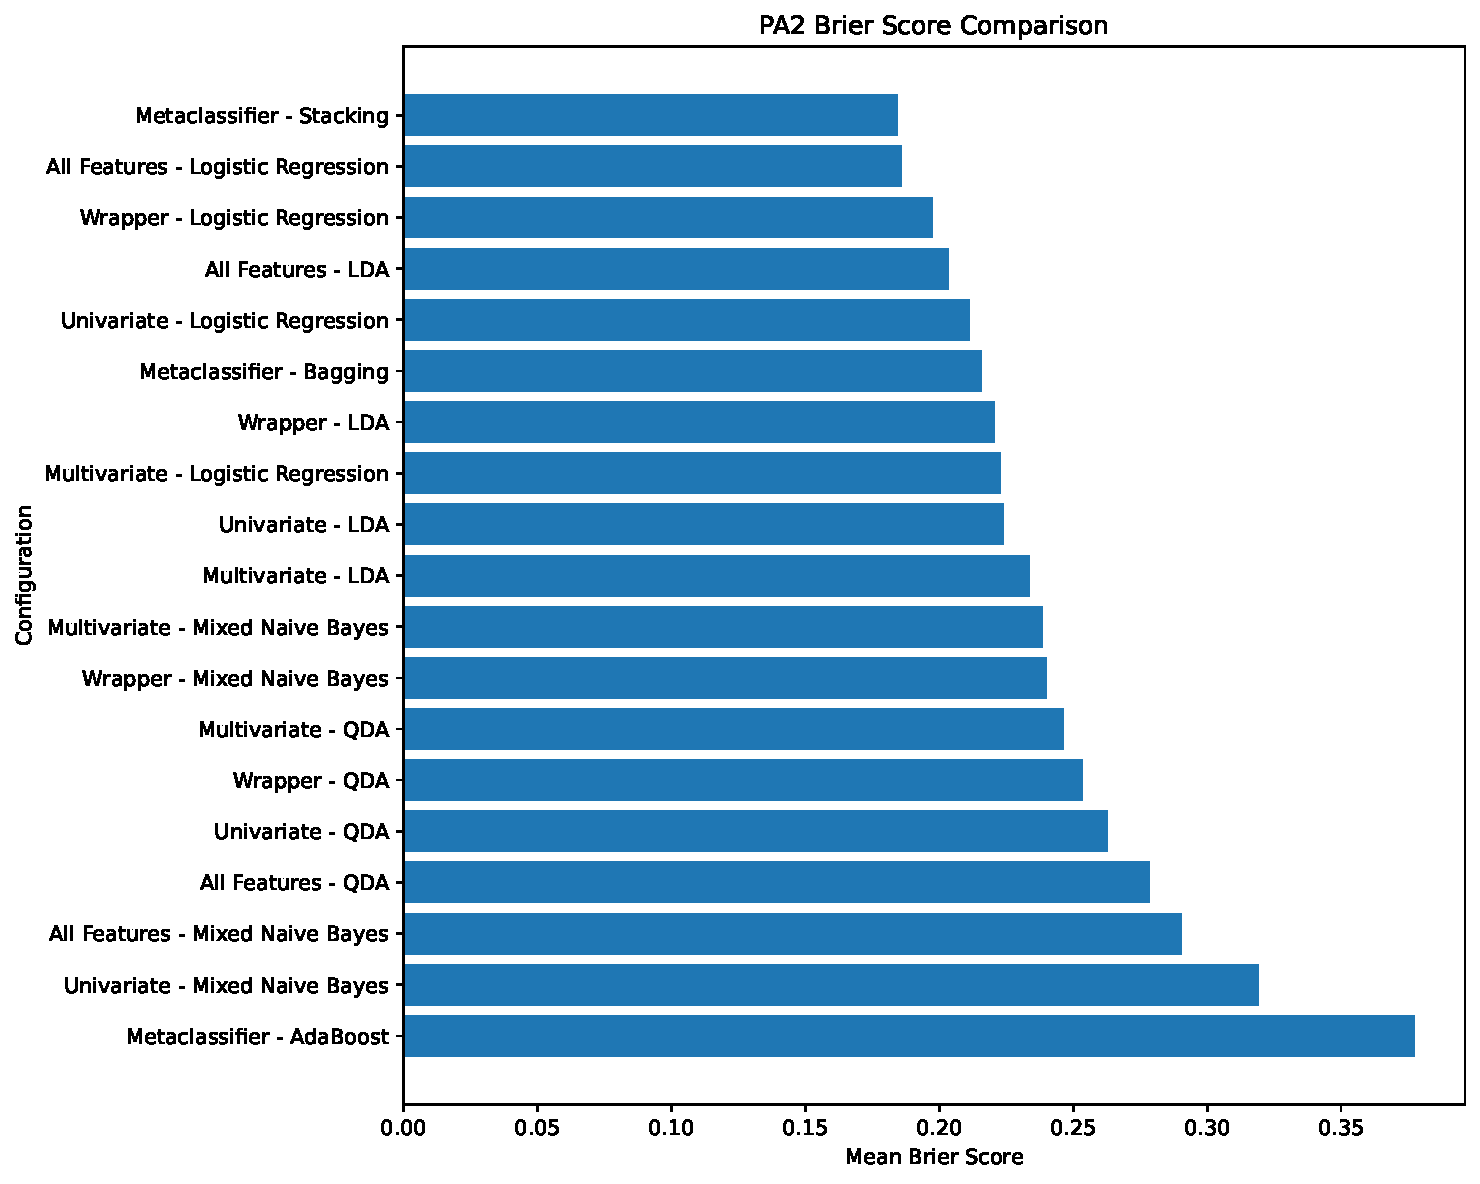
\includegraphics[width=0.76\linewidth]{../figures/pa2/brier_comparison.pdf}
\caption{PA2 mean F1 (top) and full class-probability-vector Brier score (bottom). Higher F1 and lower Brier are preferable.}
\label{fig:pa2-comparison}
\end{figure}
\clearpage

\section{Discussion}
\subsection{PA1 Performance and Dimensionality}
The imbalance explains why accuracy must be considered alongside minority-class metrics. The full-feature SVM combines accuracy 0.8653 and precision 0.8363 with recall 0.2241: its positive predictions are relatively precise, but it identifies only a small proportion of employees leaving. The full-feature Neural Network offers the strongest observed balance according to F1 and balanced accuracy, although recall 0.4219 still indicates substantial missed attrition cases.

Selection does not universally improve performance. K-NN benefits from univariate and wrapper selection, with the wrapper yielding its largest F1 improvement; multivariate selection instead lowers its F1. Removing dimensions can change which observations are considered neighbours, so retaining a useful subset can help this classifier. This interpretation is consistent with the observed improvements but does not establish the mechanism. Decision Tree improves moderately with the filters. All reduced Neural Network configurations lose performance relative to its complete representation, suggesting that the omitted information is useful in that experimental setting.

The filters assess feature--target association, with the multivariate filter also penalising redundancy. For example, the univariate subset retains both complementary overtime indicators, whereas the multivariate subset retains only \texttt{OverTime\_Yes}. The wrapper evaluates candidate additions through a Decision Tree's F1, so the resulting representation is linked to that estimator rather than independently optimised for every final classifier. These different criteria explain why the methods need not choose identical subsets or favour the same classifier. The 70.59\% reduction offers a more compact representation, but 15 transformed features do not necessarily represent 15 distinct employee characteristics. No selection strategy is best on every metric.

\subsection{Integrated Performance and Probability Quality}
Full-feature Logistic Regression in PA2 exceeds PA1's full-feature Neural Network in observed F1, while their recall is similar. Its additive log-odds model offers a comparatively simple probabilistic representation. Retaining all predictors allows jointly useful associations to contribute even when individual filter scores are modest; its default regularisation also limits coefficient magnitude. These properties plausibly explain its competitiveness, rather than establish the mechanism. Comparisons between PA1 and PA2 reflect both classifier and representation choices, so they do not isolate an effect of probabilistic modelling alone.

Aggressive filtering can discard complementary information. PA2's univariate ranking assesses predictors individually, while CFS favours relevance with low redundancy rather than optimising classifier F1. CFS therefore produces compact subsets but can omit information useful jointly or under a particular model representation. QDA's univariate improvement is consistent with reduced covariance-estimation demands, although it remains below Logistic Regression. Even PA2's classifier-specific wrapper does not recover the strongest complete-feature F1: greedy search bounded at 15 original predictors need not identify the most useful joint representation. PA1's counts concern transformed features, so dimensionality reductions are not directly interchangeable across applications.

Mixed Naive Bayes detects more minority-class cases than the other PA2 configurations, at the cost of lower precision and higher probability-vector error. Its conditional-independence assumption may be restrictive for related career and compensation predictors. Multiplying dependent evidence can distort estimated probabilities, although these experiments do not establish this as the sole explanation. Higher recall therefore does not imply better probability quality. AdaBoost's competitive AUC but much larger Brier similarly distinguishes ranking discrimination from accurate probability estimates.

Stacking adds an internal fitting stage and a final estimator, yet improves F1 and Brier only marginally relative to Logistic Regression, with unchanged recall and slightly lower AUC. Its related linear base learners may provide limited complementary information. Without uncertainty estimates or a formal paired comparison, these small differences do not justify claiming a meaningful advantage. Full-feature Logistic Regression is consequently competitive when balancing discrimination, probability quality and simplicity; Mixed Naive Bayes is preferable among the tested PA2 configurations when recall is the principal objective. Compact CFS subsets serve a different objective: reducing the number of recorded characteristics. No configuration dominates all objectives.

\subsection{Interpretation of Employee Characteristics}
Four predictors are selected in at least eight folds by both PA2 filters: \texttt{OverTime}, \texttt{JobLevel}, \texttt{StockOptionLevel} and \texttt{YearsAtCompany}. Overtime describes working conditions; job level describes organisational position; stock-option level represents a compensation attribute; and company tenure describes experience within the organisation. Their recurrence indicates that these complementary aspects repeatedly support predictive discrimination under different selection criteria. It does not establish that any attribute causes attrition, nor does selection alone reveal the direction or magnitude of an association. Overtime and stock-option level also appear in all three PA1 descriptive selections.

PA2's stable univariate selections further retain age, job role, involvement, monthly income and career-experience variables, supporting a multidimensional predictive interpretation. Relationships between professional level, compensation and experience also caution against interpreting each selected variable independently. PA1 agreement counts below come from separate full-data fits, whereas PA2 frequencies count outer training-fold selections. The latter indicate recurrence under overlapping resamples, not independent replication or a causal importance ranking.
The repeated original variables describe several complementary aspects of the employee context. \texttt{BusinessTravel} and \texttt{OverTime} concern working conditions; \texttt{JobInvolvement} records involvement in work; and \texttt{JobRole} distinguishes professional functions. \texttt{MonthlyIncome} and \texttt{StockOptionLevel} describe compensation, while \texttt{MaritalStatus} describes personal circumstances. Their selection by all three strategies identifies recurring associations relevant to classification in this dataset, without establishing causal effects or the direction of each association.

The existing descriptive analysis provides context for overtime: attrition is 30.53\% among employees with overtime and 10.44\% among those without it. These rates support interpreting overtime as associated with attrition-related classification patterns, rather than as a cause of leaving. \texttt{Age}, \texttt{JobSatisfaction}, \texttt{NumCompaniesWorked} and \texttt{TotalWorkingYears}, each selected by two strategies, add demographic, satisfaction and career-experience information.

Dummy categories must be interpreted together at original-variable level. For example, \texttt{OverTime\_Yes} and \texttt{OverTime\_No} encode the same employee characteristic; different retained \texttt{JobRole} categories still refer to job role. Agreement across methods makes the selected representation easier to discuss, but does not by itself provide a ranked importance measure or explain individual Neural Network predictions.

\subsection{Limitations}
The IBM dataset is synthetic/fictitious, so these findings should not be treated as evidence about a specific real workforce. Class imbalance remains present and minority-class recall is limited. Hyperparameters and decision thresholds were not optimised; conclusions concern the chosen configurations. PA1 fixes reduced subsets at 15 transformed features; PA2 ranks or searches original predictors, retaining at most 15. Neither setup establishes a globally optimal subset.

Numerical nominal codes in standalone LDA/QDA introduce representation dependence without meaningful ordering. QDA's instability inside stacking illustrates the sensitivity of covariance estimation to the available representation and sample size. PA1's wrapper and PA2's stacking fit preprocessing before their internal folds, as disclosed in Methodology; outer held-out folds remain excluded from all fitting. Cross-validation provides honest estimates for fixed configurations, but choosing the highest observed mean among many configurations may favour sampling variation. No independent external validation or statistical significance claim is provided. Logistic Regression's form is comparatively interpretable, but no fitted coefficient analysis is reported here; selection describes retained information rather than explaining individual predictions.

\section{Conclusion}
PA1 and PA2 address one attrition-prediction problem using honest stratified cross-validation, with outer held-out data excluded from preprocessing, feature selection and model fitting. The full-feature Neural Network leads PA1 in F1, while probabilistic Logistic Regression and Stacking are particularly competitive across the integrated comparison. Stacking's F1 and Brier gains over Logistic Regression are marginal; Mixed Naive Bayes provides the highest PA2 recall.

Feature selection reduces dimensionality and benefits some classifiers but does not systematically improve the strongest complete-feature models. Repeated retention of overtime, job level, stock-option level and company tenure in PA2, together with recurring PA1 characteristics, supports interpretation of predictive associations without causal claims. The practical choice therefore depends on the trade-off between predictive performance, sensitivity to attrition, dimensionality and model complexity.

\begingroup
\small
\raggedright
\bibliographystyle{plain}
\bibliography{references}
\endgroup
\end{document}
